\chapter{Design del Sistema}
\raggedright{\section{Analisi dell'architettura e motivazioni}}
L'architettura del software precedente era strutturata in maniera tale che fosse monolitica: era composta da tre strati gerarchici, dove il più basso, la View, era il \gls{layer} deputato al \gls{front end}, il layer centrale, i Model, era deputato alla gestione dei modelli richiesti dal sistema e infine il layer Database, che gestiva la manipolazione dei dati ed eventuale loro creazione, rimozione o modifica. \\
In Alexandria, nella fase di progettazione dell'architettura del sistema, il compito più arduo è stato quello di mantenere il Database e riutilizzare il codice sorgente ma ristrutturare l'architettura per renderla più flessibile e non monolitica, in particolare di adottare l'architettura \gls{REST}. Il sistema infatti prevede più sottoinsiemi di layer che collettivamente compongono l'applicativo: il front end è composto da tre layer, uno per la comunicazione \gls{HTTP} con il server, uno per l'interfaccia grafica e un'altra per la modellazione delle classi richieste. Il layer per la comunicazione a sua volta è composto da un layer aggiuntivo per la corretta gestione dei dati, utilizzato solamente dal front end nella trasmissione dei dati o per la richiesta di lettura. L'intero sottosistema del front end è inglobato nell'architettura \gls{REST} che comprende anche il lato server. Quest'ultimo infatti rispecchia la rappresentazione di una architettura REST basata su HTTP, dove lo stato dell'applicazione e le funzionalità sono divisi in risorse, ogni risorsa è unica e indirizzabile usando sintassi universale per uso nei link ipertestuali. Tutte le risorse sono condivise come interfaccia uniforme per il trasferimento di stato tra front end e risorse, questo consiste in un insieme vincolato di operazioni ben definite, un insieme vincolato di contenuti, opzionalmente supportato da codice a richiesta.
Abbiamo deciso di implementare un'architettura REST per la versatilità di richiedere e trasmettere le risorse al server, per la falicità del mapping del Database nelle entità e soprattuto perché perfetto per le nostre esigenze: il database durante la fase di progettazione già era implementato, ma non era completamente utilizzabile per via dell'architettura monolitica del precedente sistema. L'API Rest si è presentata come un'ottima scelta per poter implementare un nuovo sistema senza dover realizzare dal nulla lo stesso database.

\raggedright{\section{Descrizione e motivazioni delle scelte tecnologiche adottate}
Le tecnologie usate durante lo sviluppo del progetto sono essenzialmente tre: PostgreSQL per il Database Management System, Spring Boot per l'API Rest da implementare per la comunicazione con il DBMS e Flutter per lo sviluppo del front-end. Di seguito descrizione e motivazioni delle nostre scelte.

\raggedright{\subsection{PostgreSQL}}
PostgreSQL è un \gls{DBMS} di tipo relazionale in cui è possibile inserire dati, modificarli,  ricercarli ed eliminarli. E' inoltre fornito di funzionalità aggiuntive come la creazione di funzioni tramite PLPGSQL o SQL Dinamico. \\
In Alexandria, il back-end è gestito in parte da PostgreSQL. Il motivo principale di questa scelta è la già nota esistenza di un Database apposito e le modifche pensate durante la fase di progettazione non erano tali da dover reimplementare interamente il Database. Non avrebbe avuto senso dover reimplementare lo stesso database con le stesse funzioni per un nuovo DBMS, perdendo così tempo per la progettazione dell'applicativo, anche perché il Database risultava perfettamente funzionante durante la fase di testing del vecchio applicativo. \\
Il DBMS ci ha permesso di implementare funzioni apposite per determinate query, soprattutto per le relazioni ricorsive, tipi enumerativi e cast dedicati, funzionalità che magari non erano presenti in altri DBMS. \newpage
\raggedright{\subsection{Spring Boot JPA}}
\gls{Spring Boot} è un API Rest atto a implementare un applicativo capace di comunicare mediante archiettura REST. \\
In Alexandria, Spring Boot è stato uno strumento fondamentale per l'implementazione e la gestione delle risorse dal client al DBMS. Prima dell'implementazioen effettiva, abbiamo avuto dinanzi una vaste alternative di framework per l'implementazione di tale architettura. La scelta finale è però ricaduta su Spring Boot principalmente per due motivi: dato che l'applicativo originale era stato scritto in Java, ci è risultato più conveniente implementare Spring Boot su un eseguibile Java essendo possibile poter recuperare il codice sorgente originale e modificarlo all'occorrenza. Inoltre, Spring Boot offre la possibilità di effettuare query native, oltre a quelle di supporto: in tal modo abbiamo potuto riportare uno a uno le query già implementate nel vecchio sistema, senza doverle reimplementare. L'unico sforzo effettivo è stato quello di adattare le funzioni di query per ogni caso.  \\
\raggedright{\subsection{Flutter}}
Flutter è un framework open source per la creazione delle interfacce native per diversi sistemi operativi, tra cui Android. \\
Una delle motivazioni principali della scelta dell'utilizzo di Flutter è la sua enorme semplicità nella creazione e modifica delle interfacce grafiche. Inoltre, è fornito nativamente il supporto per la maggior parte dei sistemi operativi in uso, così, se si dovesse esportare Alexandria su nuove piattaforme, basterà solamente compilare il codice sorgente e distribuire l'applicativo. In caso di modifiche alle schermate in base alle esigenze del dispositivo che lo richiede, basterà modificare i metodi appositi, senza dover ricorrere ad artifizi particolari. Infine, essendo un linguaggio particolarmente simile a Java, è stato semplice dover esportare il codice originale in Flutter, modificando però opportunamente il codice in caso di incompatibilità.

\newpage

\raggedright{\section{Diagramma delle classi di design}}
Alla luce di quanto è stato detto, viene riporrtato il seguente diagramma delle classi di Design del front-end: 
\\~\\
        \begin{center}
            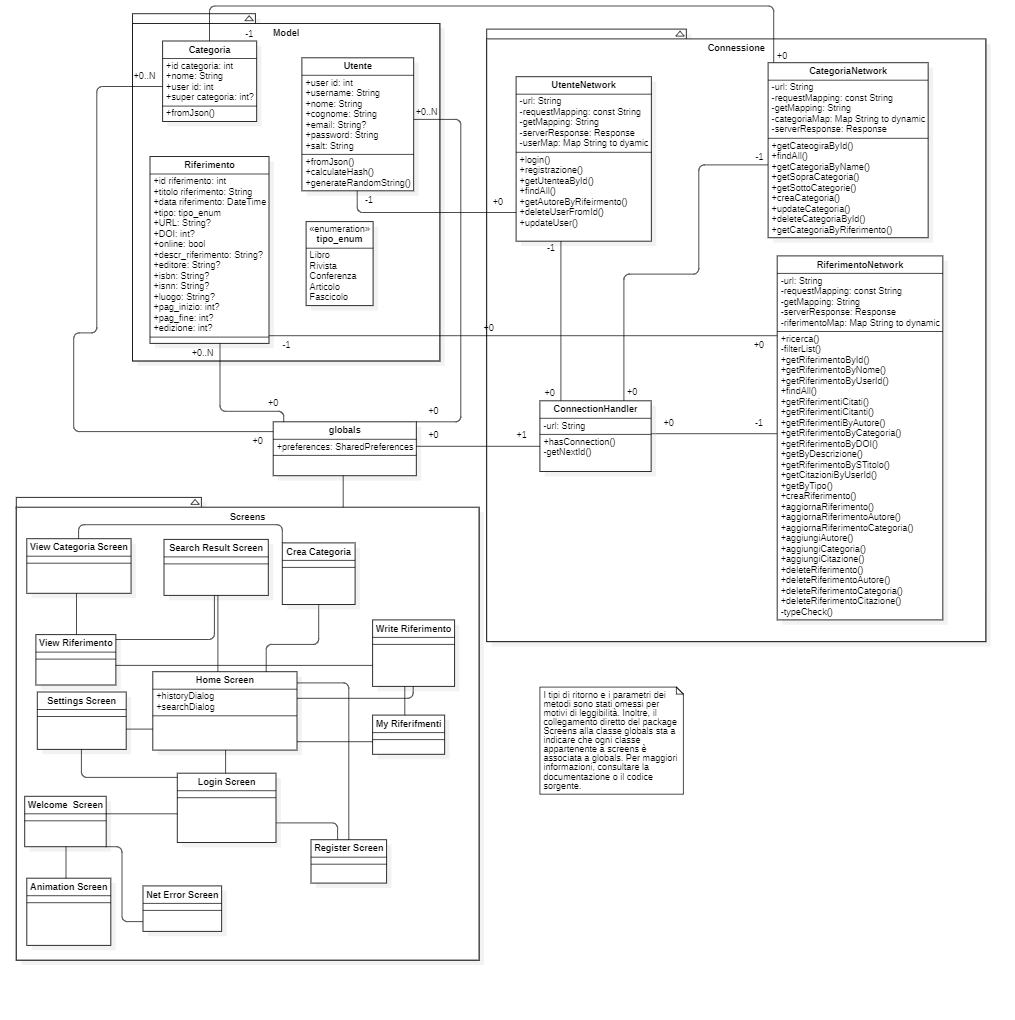
\includegraphics[width=.95\textwidth]{Immagini/Alexandria/UML Design.PNG} 
        \end{center}
L'applicativo consta in tre package principali, uno per gli Screen (GUI), uno per la connettività e infine uno per rappresentare i Model. Inoltre sono presenti classi globali come appunto \textit{globals} che fugnono da intermediario fra i package o per l'avvio dell'applicativo. In questo diagramma sono stati rappresentati in dettaglio le relazioni fra le classi e gli attributi, ma sono stati omessi i tipi di ritorno e i parametri dei metodi in maniera tale da rendere l'intero diagramma più leggibile. Se si volesse consultare in dettaglio ogni metodo utilizzato, si consiglia di leggere la sezione \hyperref[sourceCode]{apposita}. Inoltre, sono stati omessi dal diagramma anche le classi che implementano widget o componenti particolari per l'interfaccia grafica: essendo solamente classi di supporto, abbiamo considerato ridondante la loro presenza nel Class Diagram soprastante, anche perché le classi contenute nel package Screen sono autoesplicative e fanno intendere il loro funzionamento anche senza specificare le componenti che sfruttano per la loro corretta esecuzione. Infine, sono stati omessi gli attributi degli screen e i loro metodi essendo la maggior parte attributi nativi e solamente tecnici che non contribuiscono alla comprensione della visione complessiva del sistema.


\raggedright{\section{Diagrammi di sequenza di design}}
Di seguito vengono riportati i Sequence Diagram per i casi d'uso identificato nella \hyperref[casiUso]{sezione 2.3}. \\~\\
\raggedright{\subsection{Ricerca Riferimenti}}
        \begin{center}
            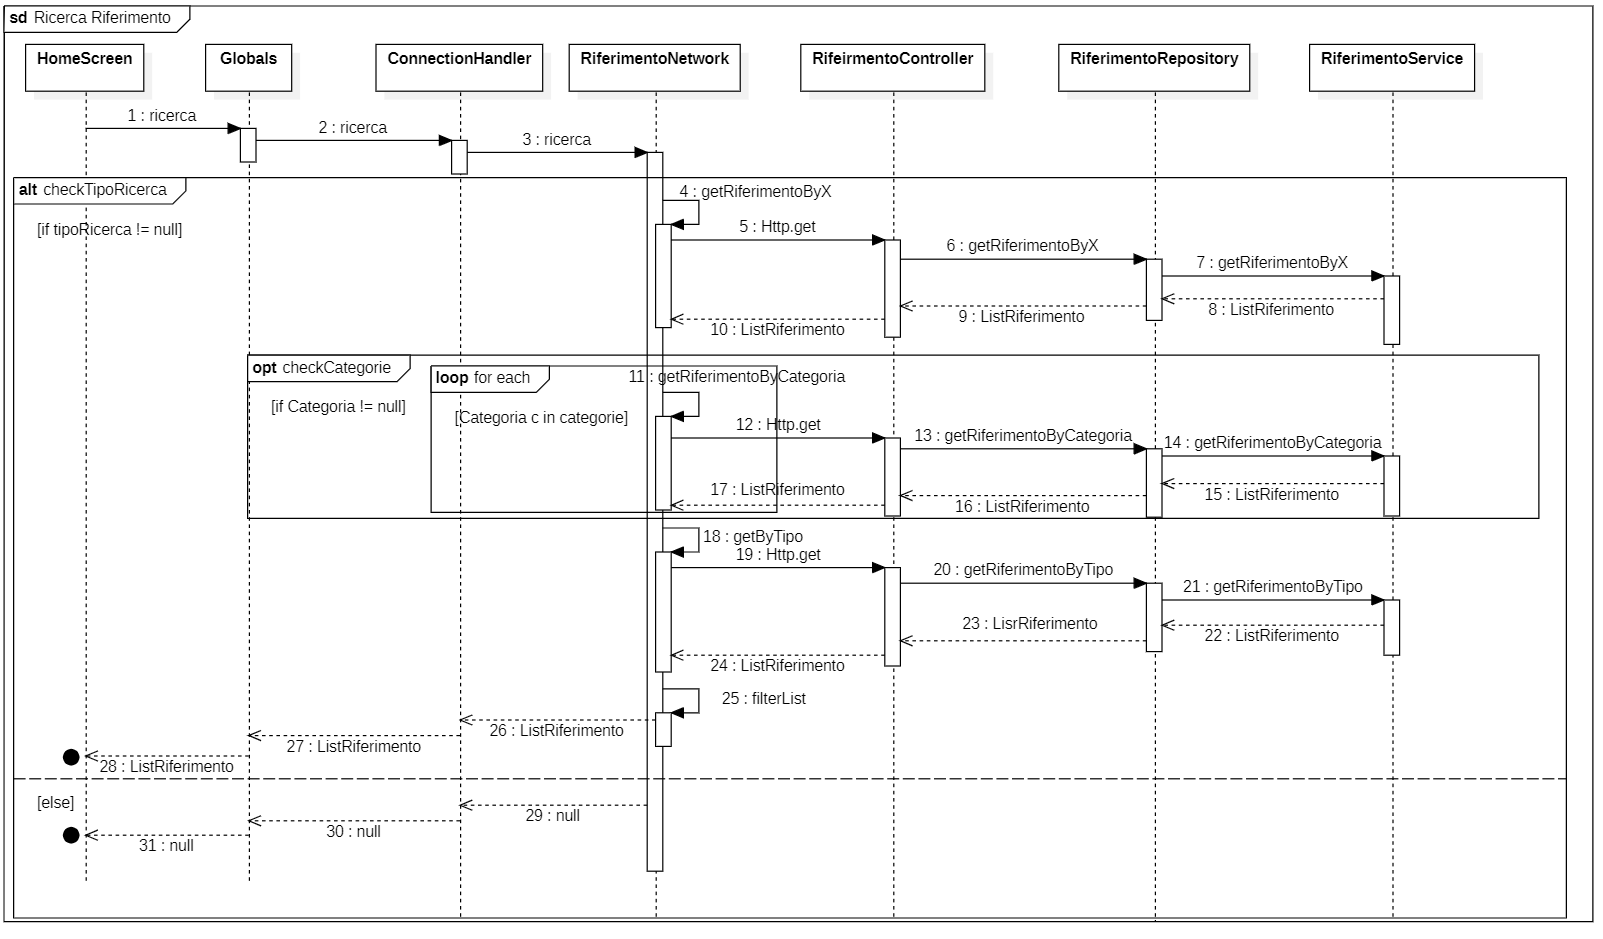
\includegraphics[width=1.0\textwidth]{Immagini/Alexandria/SequenceDesignRicerca.PNG} 
        \end{center}
Il seguente Sequence Diagram mostra le entità coinvolte durante la fase di ricerca. Da notare che sono state incluse entrambi i sottosistemi front-end e back-end. Nota: il metodo \textit{getRiferimentoByX} sta a indicare diversi metodi che hanno lo stesso nome ma che si differenziano per X, ovvero il tipo di ricerca che viene effettuata (per Titolo, per Autore o per DOI).
\raggedright{\subsection{Creazione Riferimento}}
        \begin{center}
            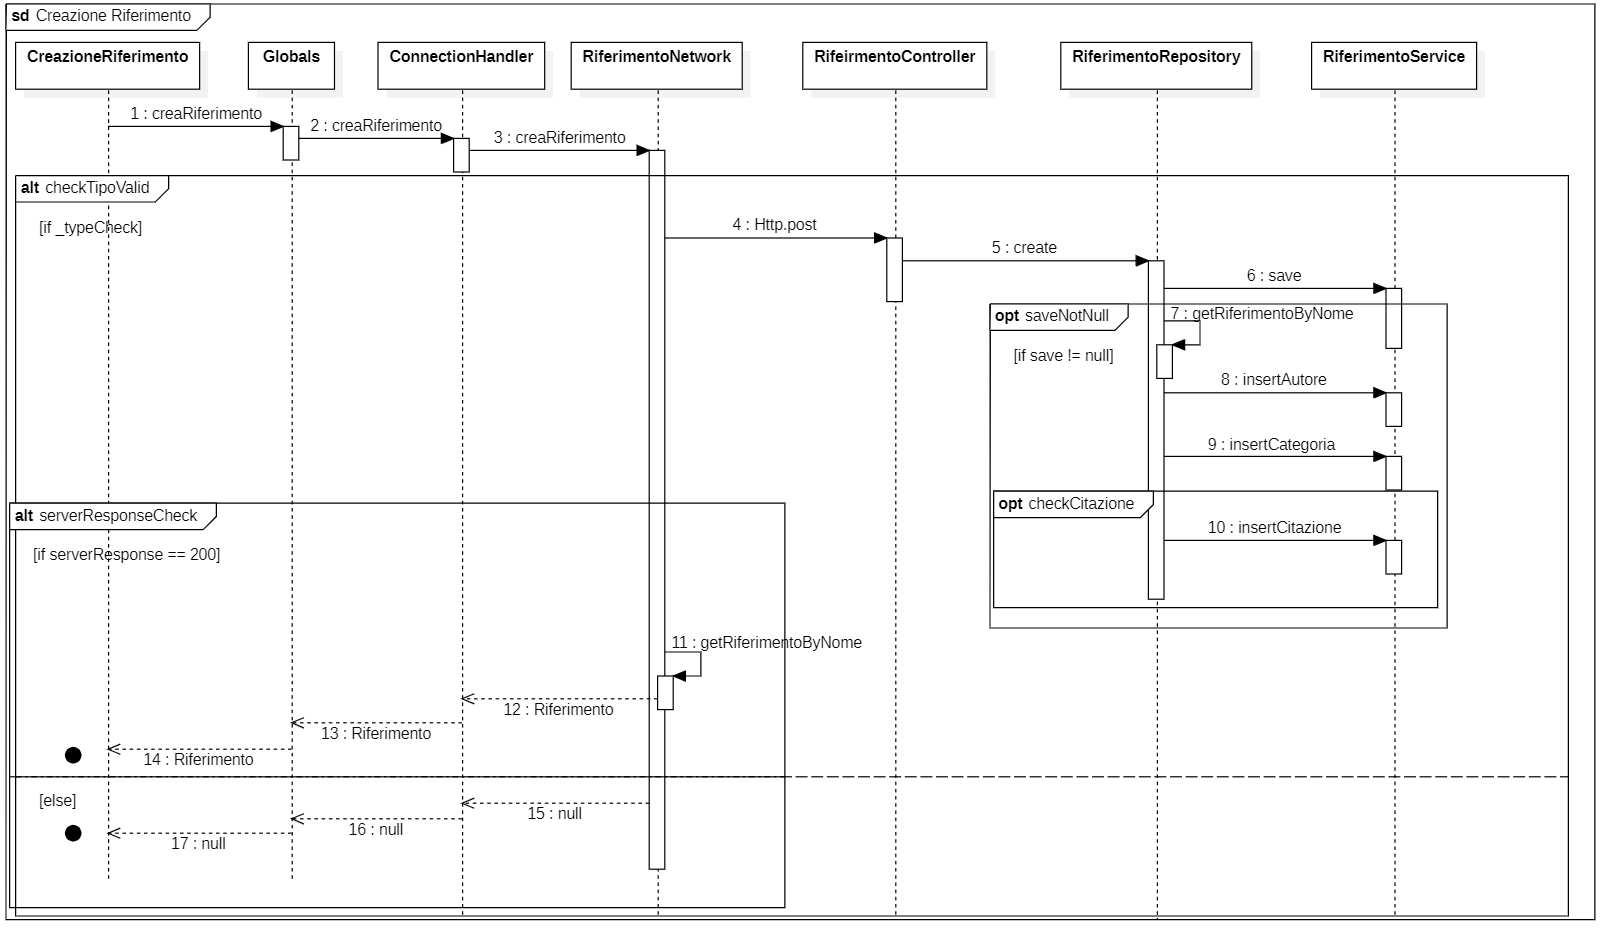
\includegraphics[width=1.0\textwidth]{Immagini/Alexandria/SequenceDesignCreazione.PNG} 
        \end{center}
Il seguente Sequence Diagram mostra le classi coinvolte durante la fase di creazione di un riferimento. Il sequence assume un comportamento diverso in base al metodo typeCheck: se l'utente inserisce valori non validi per un determinato tipo, allora l'operazione di post non viene effettuata. 
\raggedright{\subsection{Modifica Riferimento}}
        \begin{center}
            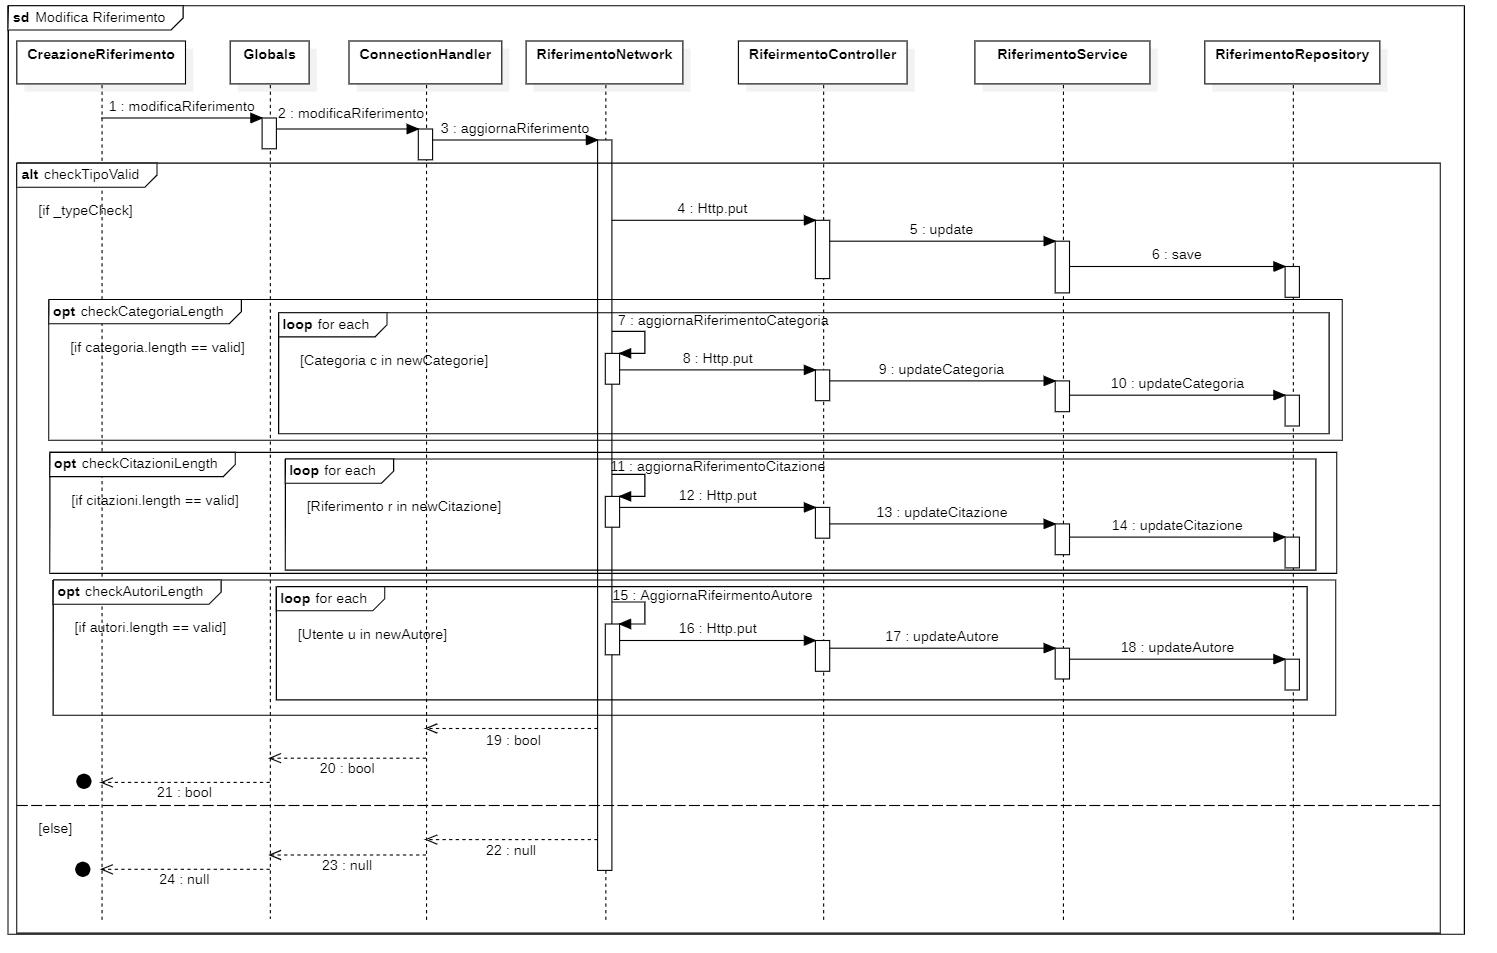
\includegraphics[width=1.0\textwidth]{Immagini/Alexandria/SequenceDesignModifica.PNG} 
        \end{center}
Il seguente Sequence Diagram mostra le classi coinvolte e i metodi coinvolti durante la fase di modifica di un riferimento. Anche in questo caso, si può notare un comportamento differente in base al check basato sui valori inseriti dall'utente. Inoltre, viene restituito un AND fra gli i vari valori modificati: se un valore, per esempio Autore, viene modificato, si effettua un controllo effettivo sulla modifica e viene restituito un AND con il riferimento modificato che restituirà il risultato finale.
\raggedright{\subsection{Creazione Categoria}}
        \begin{center}
            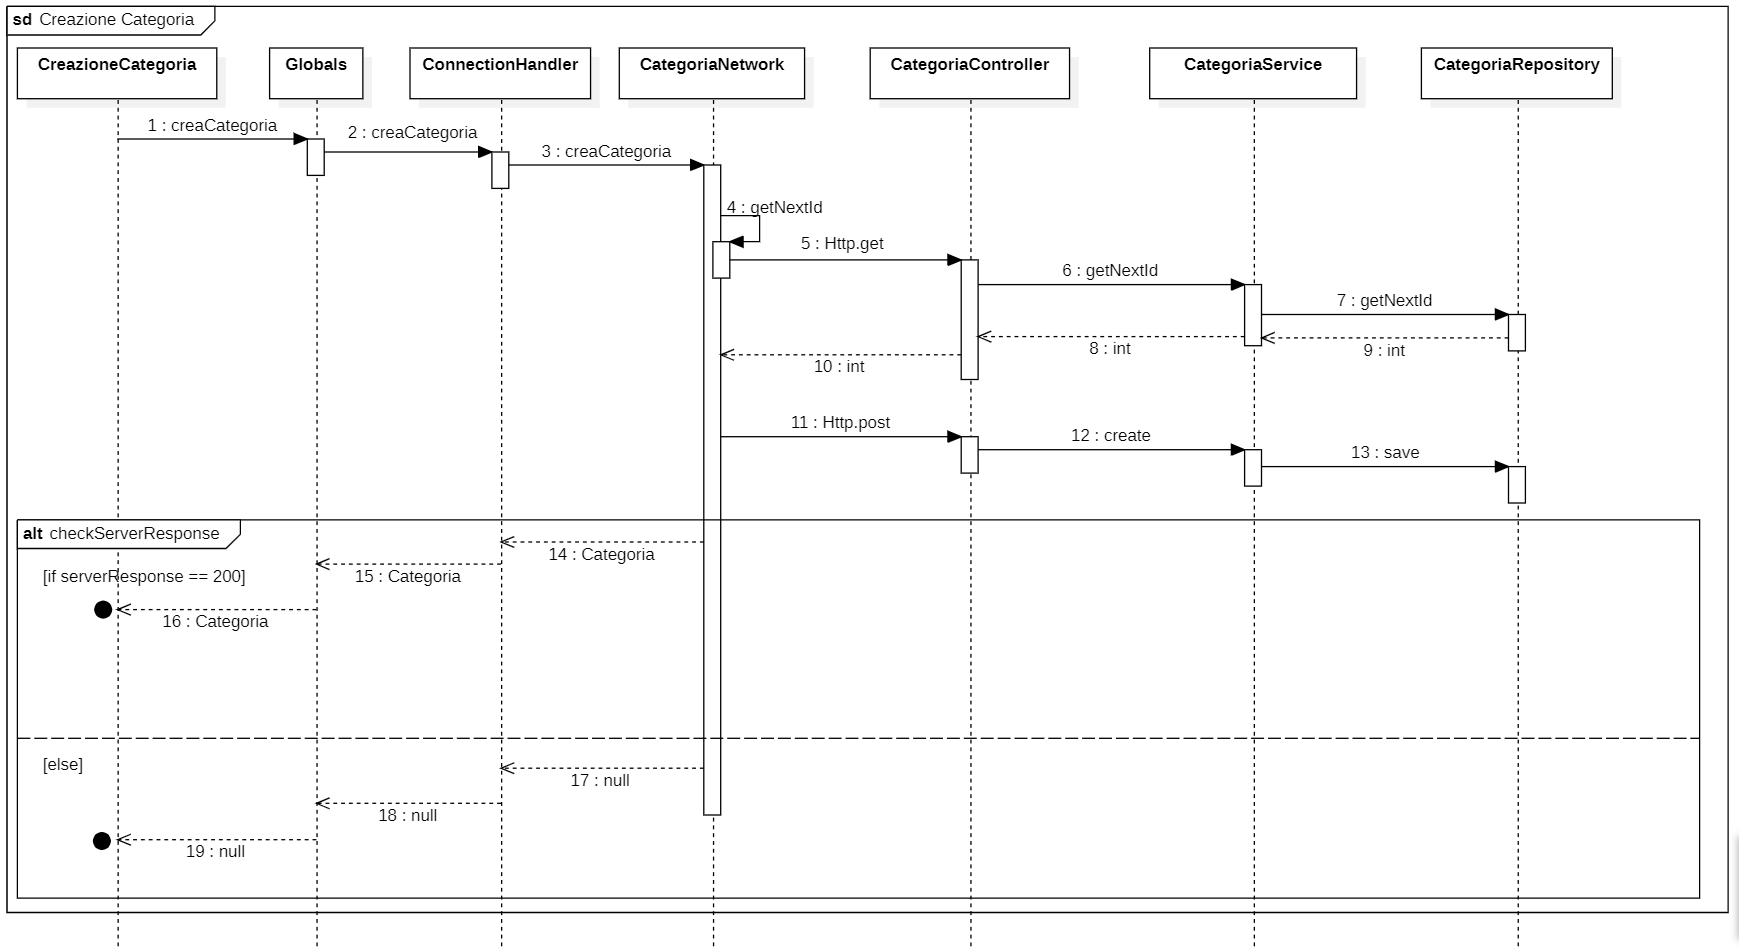
\includegraphics[width=1.0\textwidth]{Immagini/Alexandria/SequenceDesignCategoria.PNG} 
        \end{center}
Il seguente Sequence Diagram mostra le classi coinvolte durante la fase di creazione di una categoria. Non è un'operazione complessa data la natura semplice della categoria stessa, quindi non vengono effettuati particolari check sugli attributi. 



\raggedright{\section{Codice sorgente e Dockerfile}}
\label{sourceCode}
E' possibile visionare e consultare l'intero codice sorgente, dockerfile e file vari presso la seguente \href{https://github.com/Gheovgos/Alexandria/tree/main}{repository (testo cliccabile).} In particolare, è possibile consultare il codice sorgente dell'applicativo del front-end in \href{https://github.com/Gheovgos/Alexandria/tree/main/alexandria}{questa subdirectory}, il codice sorgente del back-end in \href{https://github.com/Gheovgos/Alexandria/tree/main/alexandria%20server}{questa subdirectory} e dockerfile in \href{url}{questa subdirectory}. \\
Abbiamo cercato di rendere l'applicativo più modulare possibile in maniera tale che le modifiche da apportare in futuro, se necessario, saranno più facili da effettuare e per poter integrare nuove funzionalità con semplicità nel codice. Inoltre sono presenti nella nostra API funzioni non utilizzate per offrire supporto in futuro, se necessario.
